\section{引言}
并发程序的一次观测可以遗漏比调度顺序更多的信息。对于同一地址、同一值的多次写，读值不能确定具体来源；对于不同线程的写，线程内程序序不能确定每地址的修改顺序。Release--Acquire（RA）语义进一步允许无法解释为顺序一致交错的观测。因此，分析一段日志时，仅找到一个合法执行，并不足以回答“这个读还可能来自哪些写”或“修改哪一项记录即可消除冲突”。后两类问题需要在既有记录约束下，对原始来源与写序选择求\emph{完整支持}。

一般 RA 一致性问题已经具有复杂的计算边界。最近的结果表明，每地址单写者时可多项式判定，而允许两写者后一般情形仍为 NP-hard~\cite{govind2026}。另一方面，给定 reads-from（RF）关系后判定是否存在合法写序，已有高效算法~\cite{tunc2023}。这两类结果都提示我们：应明确哪些信息已知、哪些选择保留，而不能把“弱内存一致性”视为一个统一的输入合同。本文保留 RF 和 coherence order（CO）两类原始选择，并允许反复添加、撤销针对这些选择的假设。

一个自然路线是将所有合法补全编译为可重复查询的表示。困难出现在编译之前：即使每个实际执行只使用局部的通信边，\emph{全部候选边的并图}也可能很宽。仅从必选 RF 边推导同步，会遗漏所有来源共同保证的因果关系；反过来，将同值发布合并，又会删除诊断所需的来源身份。已有关系分析提供 may/must 上下界和语义过滤接口~\cite{haas2023}，但其一般可靠性结论不会直接给出具体程序族上的候选跨度与接口界。

本文回答以下问题：\emph{在不固定来源身份、不预选 CO 总序的情况下，哪些可检查的发布结构足以保证整个候选表示具有有界接口？该界是否能服务于一个需要完整支持的任务？} 我们考虑有限、完整的阶段观测：每个线程在本轮多次发布相同交替位，随后读取入邻居的上轮位；每轮事件密度和每地址写覆盖间隔有界。多次发布之间可以插入数据写，因此它们的同步效果不同。

主要结论由一条具体推理链组成。首先，完整的交替读序列与单写者标志的 coherence 将来源\emph{块号}锁定为上一轮，却不固定块内来源。其次，块首发布是每个候选来源的共同前序，因而必然先于等待。最后，这些共同前序沿同步网络传播，排除过远 RF、固定远距离 CO，并使固定 CO 的覆盖边也具有有界跨度。后一步需要写覆盖假设；只缩短 RF 或未决 CO 尚不足以约束整个表示。

本文有三项贡献。
\begin{enumerate}
\item 给出来源未定发布网络的局部化定理及完整证明。若网络有向直径为 $d$、每阶段至多 $b$ 个非初始化事件、写覆盖间隔为 $G$、初始化写数为 $a$，则二元选择布局的事件袋大小至多 $(4d+G+3)b+a$，与阶段总数 $n$ 无关。定理约束候选并图，而不是一个已经选定的执行。
\item 将该结构结果接入保持原始标签的联合端口编译，明确二元选择与原子 RF 分组的不同参数界。实例中，旧单例核的候选图包含 $K_{n,n}$，共同来源核则具有统一界；一个身份敏感的 CO 查询说明，不能通过合并同值来源获得这个结果。通用自动机、后缀商和传播编码不作为新的核心贡献。
\item 实现来源日志的全部单字段修复，并提供原生分析对照、不同同步拓扑、独立语义核对和可复现制品。实验的目的在于检验定理能否解释实际候选结构、完整支持是否有用以及编译在何处失效，而非宣称全面优于成熟验证工具。
\end{enumerate}

\section{动机：同值发布并不具有相同支持}\label{sec:motivation}
考虑两个线程交换共享状态的有限内核。线程 A 在一次阶段内先写 $x$，发布标志 $f_a$，再写 $y$，随后再次发布\emph{相同}标志值。线程 B 执行对称操作，并在下一阶段读取 A 的标志。两次发布分别覆盖第一项和两项数据更新；从读到的位值无法判断 B 获得了哪部分同步。这种“分段更新、同值通知”的结构保留了弱同步和竞争写入。

图~\ref{fig:identity} 抽取两轮版本载荷实例中的相关事件。设 $u$ 是 A 第一轮对 $y$ 的写，$a_0,a_1$ 是其早、晚发布，$v$ 是 B 第二轮对 $y$ 的写，$r$ 是 B 的等待，$s$ 是其随后对 $y$ 的读。定义原始文字
\[
 d=\RF(v,s),\quad e=\RF(a_0,r),\quad
 \ell=\RF(a_1,r),\quad q=\CO(u,v).
\]
两个发布都写 1；两位线程在第二轮都对数据写 2，因此数据读的来源身份也未由值唯一决定。

\begin{figure}[tb]
\centering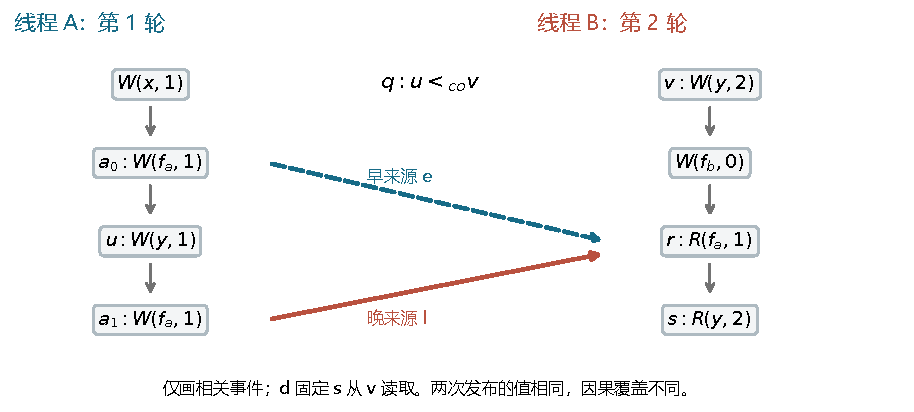
\includegraphics[width=\textwidth]{identity_example.pdf}
\caption{身份敏感的同步。虚线和实线是互斥的 RF 选择，并非同时存在的边；省略的事件仍属于完整输入。}\label{fig:identity}
\end{figure}

在 $\{d,\ell\}$ 下，有
\[
u\;\SB\;a_1\;\RF\;r\;\SB\;s.
\]
由于 $s$ 从 $v$ 读取，write--read coherence 强迫 $u<_{\CO}v$。选择早发布 $a_0$ 时，上述因果链不存在；不仅无法用这条链证明 $q$，实际上 $q$ 的两个方向都有合法补全。表~\ref{tab:motivation} 展示同一个编译结果上的查询、冲突与撤销。附录~\ref{app:witness} 给出允许 $\neg q$ 的完整见证，避免以“未推导出”代替“确有支持”。

\begin{table}[tb]
\caption{同值来源改变 CO 支持。支持是存在合法完整补全，而非静态近似。}\label{tab:motivation}
\centering\begin{tabular}{lll}\toprule
原始假设 $\alpha$ & 一致性 & $q$ 的支持\\\midrule
$\varnothing$ & SAT & 真、假均可\\
$\{d,e\}$ & SAT & 真、假均可\\
$\{d,\ell\}$ & SAT & 仅真\\
$\{d,e,\neg q\}$ & SAT & 仅假\\
$\{d,\ell,\neg q\}$ & UNSAT & 无支持\\
$\{d\}$（撤销来源） & SAT & 真、假均恢复\\\bottomrule
\end{tabular}
\end{table}

这个例子区分了两种知识：$a_0$ 作为块首发布，在任一来源选择下都先于 $r$；但 $u$ 是否先于 $r$ 取决于来源身份。前一种知识适合永久认证和缩小候选表示，后一种相关性必须留在精确查询中。仅保存必选 RF 无法获得前者，合并 $a_0$ 与 $a_1$ 则破坏后者。本文所说的“必要性”是这两个具体不足的反例，不意味着所有正确算法都必须采用本文规则。
